\subsection{三択の時刻を提示する画面}
この画面では三択の時刻と，それぞれの時刻への投票数を表示する．
実際の画面を図\ref{fig:selectDisplay}に示す．
この画面への遷移時には音声による通知を行い，画面表示の変化に気づきやすくしている．
また，投票状況を時刻横に丸の数として反映し，他の人の投票を参考に帰宅時刻の検討や変更ができる設計としている．
現在時刻が投票締切時刻をすぎた際に最多投票の時刻を提示する画面へと自動的に遷移する．

\begin{figure}[htb]
  \centering
  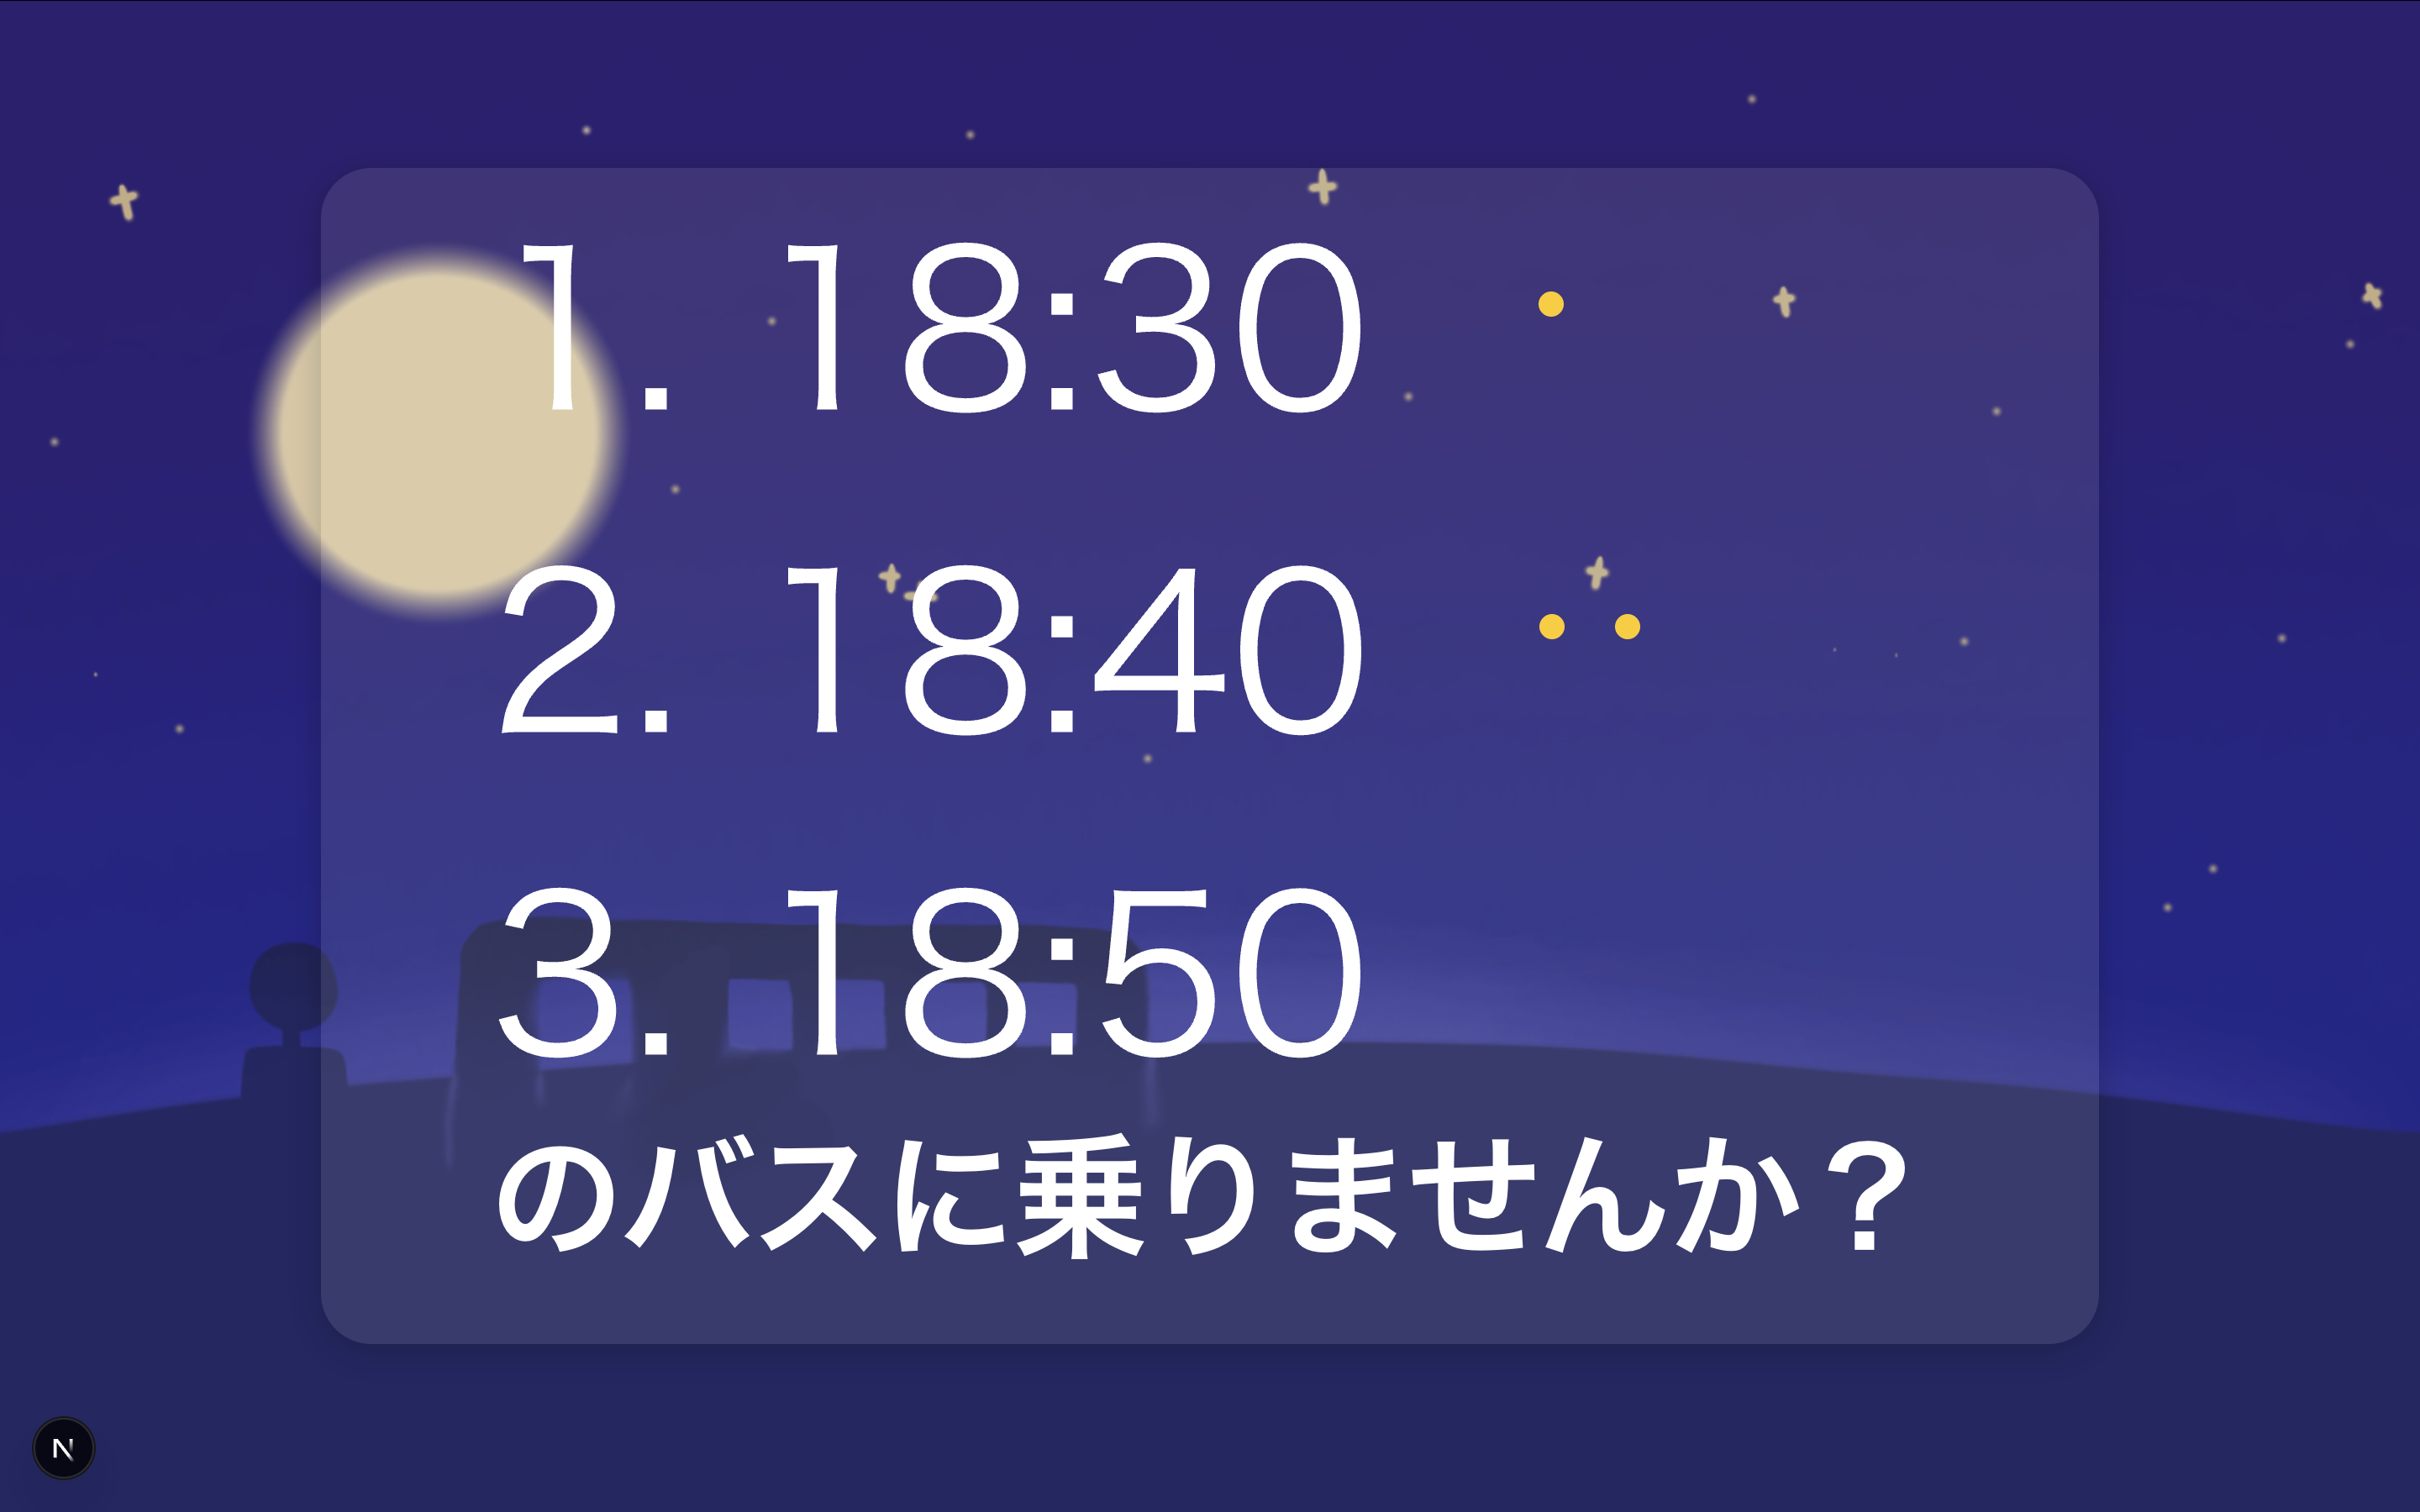
\includegraphics[width=0.7\linewidth]{selectDisplay.png} % suzuki
  \caption{三択の時刻を提示する画面}
  \label{fig:selectDisplay}

\end{figure}

本画面の設計にあたっては，設置環境や利用状況を踏まえた視認性および理解のしやすさに配慮した．
本画面は，共有スペースに設置された小型のモニターでの利用も想定し，離れた位置からでも内容を把握できるよう，時刻情報を画面内で大きく表示する設計とした．
また，各選択肢には数字を対応させ，ユーザが直感的に投票操作を行えるようにした．
加えて，「〜のバスに乗りませんか？」という表現を用いて，提示している時刻とバスの出発時刻の対応を一目で理解できるよう工夫した．
各時刻への投票状況は具体的な人数を数値で表示するのではなく，点の数として視覚的に表現した．
これにより，他者の選択傾向を直感的に把握できる一方で，人数の多寡を過度に強調せず，選択に対する心理的な圧力を和らげる意図がある．

また，本システムでは画面遷移への気づきを促すための一手段として音声通知を併用した．
通知に用いる音声には読み上げソフトである音読さん\cite{ondoku}を利用して作成した．
具体的には，「おすすめのバスの時刻が設定されました」という短い文言を読み上げた音声を用い，三択の提示画面へ遷移するタイミングで再生する．
音声内容は，ユーザに対して新たな情報提示が行われた事実のみを簡潔に伝える設計とし，周囲で行われている既存の対面コミュニケーションを過度に遮らないよう配慮した．
音声は画面遷移への気づきを促す目的で用い，具体的な時刻情報は表示画面に集約する設計とした．

この音声通知の作成にあたっては，画面遷移への気づきを促しつつも，通知時間が過度に長くならないよう配慮した．
具体的には，読み上げ音声の再生速度を標準よりやや速い設定とし，短時間で内容を伝えられるよう調整した．
また，周囲の環境音の中でも認識されやすいよう，比較的高めの声色を選択して音声を作成した．
以上のように，本システムにおける音声通知は，画面表示を中心とした情報提示を補完する手段として位置付けている．